\documentclass{base}
% Dateikodierung ist utf8
\usepackage[utf8]{inputenc}
\usepackage{url}
\usepackage[export]{adjustbox}
\usepackage{amsmath}
\usepackage{listings}
\usepackage{tikz}
\usepackage{tabularx}
\usepackage{color,colortbl}
\usepackage{ulem}
\usepackage{pdfpages}
\usepackage{ wasysym }
\usepackage{ booktabs }
\usepackage{lscape}
\usepackage{multicol}
\usepackage{longtable}
\usepackage{flexisym}

\begin{document}

\Abgabeblatt{Assignment 7}{28.5.2018}{????}{????}{Yannis Rohloff (yannis@uni-bremen.de)}{Meng Liu(lium@uni-bremen.de)}{Islam Abushanab(is\_ab@uni-bremen.de)}

\lstset{
    language=Python,
    basicstyle=\ttfamily\small,
    aboveskip={1.0\baselineskip},
    belowskip={1.0\baselineskip},
    columns=fixed,
    extendedchars=true,
    breaklines=true,
    tabsize=4,
    prebreak=\raisebox{0ex}[0ex][0ex]{\ensuremath{\hookleftarrow}},
    frame=lines,
    showtabs=false,
    showspaces=false,
    showstringspaces=false,
    keywordstyle=\color[rgb]{0.627,0.126,0.941},
    commentstyle=\color[rgb]{0.133,0.545,0.133},
    stringstyle=\color[rgb]{01,0,0},
    numbers=left,
    numberstyle=\small,
    stepnumber=1,
    numbersep=10pt,
    captionpos=t,
    escapeinside={\%*}{*)}
}


\section*{Exercise 1 of last Week:}

As we've seen earlier in the course we can encode circuits in cnf.
We can use this to encode our given problem.

First, we encode the circuit itself. The entire sorting network. with the input variables $x_0,\dots,x_5$ and the output variables $x'_0,\dots,x'_5$. Furthermore we have some intermediate variables that encode the inner nodes.
With this we can check if the network is satisfiable, which of course it is with our further constraints. Even for all possible partial valuations of $x_0,\dots,x_5$.

\sout{We add a negated version of the phase encoding, such that we search any possible solution of input variables that causes the output variables to be unsorted. If the formula then is satisfiable we know of at least one case which is sorted in the wrong order.} (We did it differnt, see below)

To build our cnf, we are using the following helper variables:
\begin{center}
	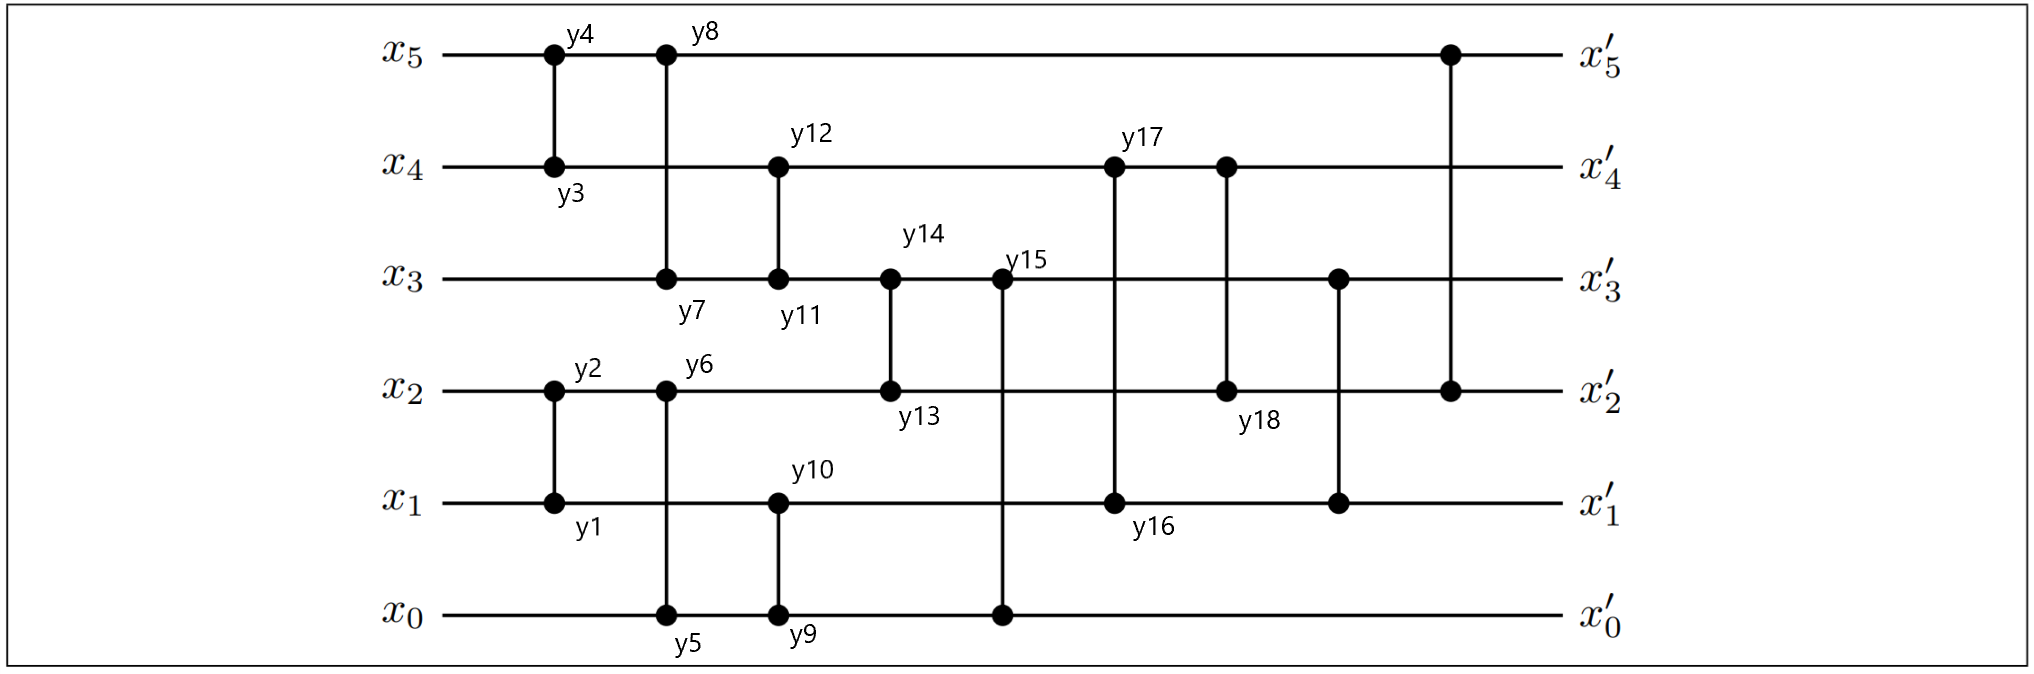
\includegraphics[width=\linewidth]{sorting_network.png}
	%\caption{Sorting network with variables}
\end{center}

We encode the functionality of the sorting network as seen in the code.
We used a KV diagram to build the semantics of each swap-gate in CNF.

For example the gate from $y_1 to y_2$ is described by:
\begin{align}
(\neg x1 \lor  y2) \land   \\
(\neg y1 \lor  x1) \land  \\
(\neg x1 \lor  x2 \lor  \neg y1 \lor  \neg y2) \land  \\
(\neg x1 \lor  \neg x2 \lor  y1 \lor  \neg y2) \land  \\
(x1 \lor  \neg x2 \lor  y1 \lor  y2) \land  \\
(x1 \lor  x2 \lor  y1 \lor  \neg y2)
\end{align}



With these clauses we've encoded the circuit. Every valuation is one possible mapping from input to possibly sorted outputs.
We are only interested in unsorted outputs ($x'_1,\dots,x'_5$). An unsorted output has a pair ($x'_i, x'_{i+1}$) where $x'_i > x'_{i+1}$
This can be formulated in DNF: \\
$(x'_0 \land \neg x'_1) \lor (x'_1 \land \neg x'_2) \lor (x'_2 \land \neg x'_3) \lor (x'_3 \land \neg x'_4) \lor (x'_4 \land \neg x'_5)$


By building the truth table and then creating the CNF from it we gain the following additional clauses.

\newcommand{\veg}{\hphantom{\neg}}
\begin{align*}
    x'_0 \lor \veg x'_1 \lor \veg x'_2 \lor \veg x'_3 \lor \veg x'_4 \lor \veg x'_5 \\
    x'_0 \lor \veg x'_1 \lor \veg x'_2 \lor \veg x'_3 \lor \veg x'_4 \lor \neg x'_5 \\
    x'_0 \lor \veg x'_1 \lor \veg x'_2 \lor \veg x'_3 \lor \neg x'_4 \lor \neg x'_5 \\
    x'_0 \lor \veg x'_1 \lor \veg x'_2 \lor \neg x'_3 \lor \neg x'_4 \lor \neg x'_5 \\
    x'_0 \lor \veg x'_1 \lor \neg x'_2 \lor \neg x'_3 \lor \neg x'_4 \lor \neg x'_5 \\
    x'_0 \lor \neg x'_1 \lor \neg x'_2 \lor \neg x'_3 \lor \neg x'_4 \lor \neg x'_5 \\
\end{align*}



If the formula has a solution we know the the helper variables have a valid assignment AND the output is still not sorted correctly.
As an example see the output (and it's visualization) below the following code.

We also implemented this formula in python.
See the following code of \verb|circuit.py|


\lstinputlisting{circuit.py}
The output of \\
\verb!python circuit.py | picosat! \\
is
\lstinputlisting{circuit.solution}
and translating this solution into an image shows the unsorted output. \\
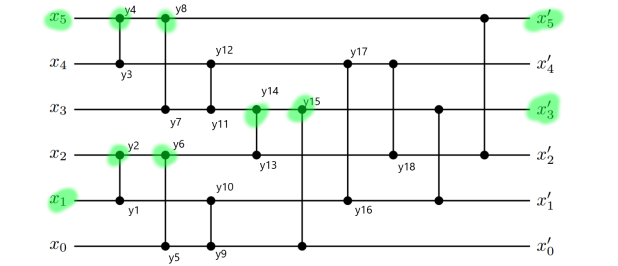
\includegraphics[scale=0.5]{sorting_network_sol.png}

Variable meanings
\lstinputlisting{circ_variables.txt}











\clearpage
\section*{Practical QBF Solving}
We define the Variables for all $i \in \{1,\dots,7, A,B\}$ and $x,y \in \{1,2,3\}$.
$$T_{(i,x,y)}$$
This variable encodes the state over all the rounds.
In the Formula we will need to constain variables to some constrains.
Since the x-player starts the turns with odd $i$'s are of the x-player and vice versa.
The round indices A and B stand for neutral rounds that fill up the last two rounds since we are ony interested in seven rounds.


To answer the question if player-x has a winning strategy it is easier to reverse it and answer the opposite.
To ask if player-x has no possible winning strategy we can check if for all possible fifth turns there exists a turn of player-o such that every possible answer of player-x results in an assignment, such that no row is a winning row.
We decided to turn the problem around since it is easier to check if there is any field different than x in a row instead of checking if all three are x.

\begin{align*}
    \exists T_{1,x,y}\dots & &&\text{|for $x,y \in \{1,3\}$}\\
    \exists T_{2,x,y}\dots & &&\text{|for $x,y \in \{1,3\}$}\\
    \exists T_{3,x,y}\dots & &&\text{|for $x,y \in \{1,3\}$}\\
    \exists T_{4,x,y}\dots & &&\text{|for $x,y \in \{1,3\}$}\\
    \exists T_{5,x,y}\dots & &&\text{|for $x,y \in \{1,3\}$}\\
    \forall T_{6,x,y}\dots & &&\text{|for $x,y \in \{1,3\}$}\\
    \exists T_{7,x,y}\dots & &&\text{|for $x,y \in \{1,3\}$}\\
    \exists T_{A,x,y}\dots & &&\text{|for $x,y \in \{1,3\}$}\\
    \exists T_{B,x,y}\dots & &&\text{|for $x,y \in \{1,3\}$}\\
    &\dots && \text{|at least one field per round} \\
    &\bigwedge_{i} \bigwedge_{x,y} \bigwedge_{x',y'} \neg T_{i,x,y} \lor \neg T_{i,x',y'} && \text{|maximum of one field at a time} \\
    &\bigwedge_{x,y} \bigwedge_{i} \bigwedge_{i'} \neg T_{i,x,y} \lor \neg T_{i',x,y} && \text{|field only used in one turn} \\
    &T_{1,1,3} \land T_{2,3,1} \land T_{3,2,2} \land T_{4,1,2} && \text{| first 4 rounds} \\
    &T_{i,1,1} \lor T_{i,1,2} \lor T_{i,1,3} && \text{| for $i \in \{2,4,6,8,A,B\}$} \\
    &T_{i,2,1} \lor T_{i,2,2} \lor T_{i,2,3} && \text{| for $i \in \{2,4,6,8,A,B\}$} \\
    &T_{i,3,1} \lor T_{i,3,2} \lor T_{i,3,3} && \text{| for $i \in \{2,4,6,8,A,B\}$} \\
    &T_{i,1,1} \lor T_{i,2,1} \lor T_{i,3,1} && \text{| for $i \in \{2,4,6,8,A,B\}$} \\
    &T_{i,1,2} \lor T_{i,2,2} \lor T_{i,3,2} && \text{| for $i \in \{2,4,6,8,A,B\}$} \\
    &T_{i,1,3} \lor T_{i,2,3} \lor T_{i,3,3} && \text{| for $i \in \{2,4,6,8,A,B\}$} \\
    &T_{i,1,1} \lor T_{i,2,2} \lor T_{i,3,3} && \text{| for $i \in \{2,4,6,8,A,B\}$} \\
    &T_{i,3,1} \lor T_{i,2,2} \lor T_{i,1,3} && \text{| for $i \in \{2,4,6,8,A,B\}$} \\
\end{align*}

<<<<<<< HEAD
$i,i' \in \{1,2,6,8,9\}, i \ne i'$\\
$k,k',k'' \in \{winshapes\}, k \ne k' \ne k''$\\
$m \in \{1,2\}$

\begin{multline*}
	\exists x_{1,i},a_{1,i}  (\bigvee \limits_{i}x_{1,i})\bigwedge (\bigvee\limits_{i, i'}(\neg x_{1,i} \lor\neg x_{1,i'}))\bigwedge(\bigvee \limits_{1, i} a_{1,i}) \bigwedge (\bigvee\limits_{1, i, i'}(\neg x_{1,i} \lor\neg x_{1,i'})) \bigwedge (\bigvee\limits_{i}(x_{1,i} \land a_{1,i})) \bigwedge \neg g_{1} \bigwedge\\
	%---------------------------------------------------------
	\forall y_{i} (\bigvee\limits_{i}y_{i}) \bigwedge\neg g_{1} \bigwedge \\
	%---------------------------------------------------------
	\exists y_{i} (\bigvee\limits_{i,i'}(\neg y_{i} \lor \neg y_{i'}))\bigwedge (\bigvee\limits_{i}((y_{i}\lor a_{1,i})\land (\neg y_{i}\lor a_{1,i}))) \bigwedge \\
	%---------------------------------------------------------
	\exists x_{2,i}, a_{2,i}(\bigvee\limits_{i}x_{2,i}) \bigwedge (\bigvee\limits_{i,i'}(\neg x_{2,i} \lor \neg x_{2,i'})) \bigwedge (\bigvee\limits_{i}a_{2,i})\bigwedge (\bigvee\limits_{i,i'}(\neg a_{2,i}\lor \neg a_{2,i'})) \bigwedge (\bigvee\limits_{i}(x_{2,i}\land a_{2,i})) \bigwedge\\
	%------------------------------------
	(\bigvee\limits_{i}((x_{1,i}\lor x_{2,i})\land (\neg x_{1,i} \lor \neg x_{2,i}))) \bigwedge (\bigvee\limits_{i}((x_{2,i}\lor y_{i})\land (\neg x_{2,i}\lor \neg y_{i}))) \\
	%------------------------------------
	\bigwedge \limits_{k,k',k'',m}(x_{m,k}\land x_{m,k'}\land x_{m,k''})\\
\end{multline*}

First line, in round 1, the cross player $x$ chooses a cell $i$, then adds to the occupied cells $a$, game is not over $g_{1} = false$.\\
Second line, the circle player $y$ does anything, the game is not over $\neg g_{1} = true$.\\
Third line, making sure the circle player made a valid move.
Fourth line till end, in round 2, the cross player $x$ chooses an empty cell $i$, then he/she wins.

=======
If the formula is satisfiable we know that all possible 5th turns results in no winning strategy, since there always is a 6th turn (player-o) such that there is no winning 7th turn for player-x.
Thus: if the formula is \textbf{satisfiable}, there is \textbf{no winning strategy}.

If the formula is unsatisfiable, there is at least one 5th turn, such the $\forall$ does not hold. This 5th turn has no counter in turn 6 that would prevent player x from winning.
So, if the formula is \textbf{unsatisfiable} player-x \textbf{has a winning strategy}.

\clearpage
>>>>>>> 62edbcac9d4be2c912840b46d9001cc9a9b9066c
\section*{Linear Programming}

The solution is really straightforward.
We have real variables $x_0,\dots,x_5$ descring the percentage of an alloy in the mix.
We mimimize the sum of the weighted costs while keeping the total sum of parts in the mix at 100\%.
Starting on line three are the clauses that ensure that the mixture is in the given bounds.
\lstinputlisting{alloy.lp}
With the solution of lp\_solve:
\lstinputlisting{alloy.lp.solution}


\end{document}
